\documentclass[11pt,journal,compsoc]{IEEEtran}
\usepackage{amsmath, cite, graphicx, color, amssymb, mathtools}
\usepackage{notation}

\begin{document}
	\title{Multi-Agent Exploration\\ with Random Network Distillation}
	
	
	\author{Philip~Raeisghasem% <-this % stops a space
		\IEEEcompsocitemizethanks{\IEEEcompsocthanksitem Philip Raeisghasem is with Louisiana Tech University, Department of Cyberspace Engineering.\protect\\
			E-mail: par019@latech.edu}}
	
	
	
	% The paper headers
	\markboth{STAT~621~Project~Report,~January~2019}%
	{Raeisghasem: Multi-Agent Exploration with Random Network Distillation}
	
	
	
	\IEEEtitleabstractindextext{%
		\begin{abstract}
			A significant part of reinforcement learning is ensuring adequate exploration. An agent cannot learn how good a new strategy is if the strategy is never tried. For multi-agent tasks, the space of possible configurations grows exponentially with the number of agents. This larger space is much harder to explore. In this paper, we apply the recently proposed Random Network Distillation exploration method to a multi-agent setting. We compare this approach to other exploration methods in the multi-agent setting. We do this both by explicitly quantifying amount of exploration and by analyzing downstream performance.
		\end{abstract}
		
		% Note that keywords are not normally used for peerreview papers.
		\begin{IEEEkeywords}
			reinforcement learning, multi-agent, exploration, random network distillation.
	\end{IEEEkeywords}}
	
	% make the title area
	\maketitle
	\IEEEdisplaynontitleabstractindextext
	\IEEEpeerreviewmaketitle
	
	
	\section{Introduction}
	\IEEEPARstart{R}{einforcement} learning is a paradigm of machine learning alongside supervised and unsupervised learning. It is most applicable to problems that can be framed as an agent acting within an environment to achieve some goal. Like supervised learning, reinforcement learning happens through a feedback mechanism during an initial training phase. Unlike in supervised learning, this feedback is not in the form of `labeled' data. There are no simple `correct' answers to directly compare the model's performance against. Instead, the feedback loop in reinforcement learning is between the agent and the environment by way of a reward function. Broadly speaking, instead of learning whether its actions are `right' or `wrong', the agent learns how good its actions are. 
	
	This difference in feedback mechanism is important for allowing reinforcement learning models to learn from self-generated experience. Thanks to the advent of deep neural networks, the space of problems solvable by artificial intelligence and machine learning has exploded in size. Many of these problems, however, require much more data to solve. In supervised learning, vast datasets that require significant preprocessing are the norm, and a human is needed to label every single training example. In contrast, a human often need only specify the reward function for a given environment in reinforcement learning. 
	
	While for many problems it can be challenging to design a reward function that will lead to desired behavior, a large class of problems are amenable to very simple and sparse reward functions. If the problem is a two-player game, for example, the agent could only be rewarded at the very end, depending on whether it won the game. Using these sparse reward functions comes at the cost of the agent receiving less feedback. That is, there is a tradeoff between difficulty and human effort in embedding prior knowledge. This tradeoff is not unique to reinforcement learning, but it has given rise to unique methods in reinforcement learning for addressing the issue.
	
	In particular, using a sparse reward function exacerbates the existing problem of exploration. While learning, an agent must always be deciding how confident it is in its current strategy. If it is very confident in the information it has received so far, it will choose to act in ways that have given it large rewards in the past. The agent is said to be exploiting its current knowledge. If the agent is not very confident, it may decide to try something new in order to gather information. The agent is then said to be exploring the environment. A sparse reward function lessens the effectiveness of exploration by limiting the number of times an agent is given any feedback after exploratory actions.
	
	The difficulty of exploration depends on more than just the sparsity of the reward function, of course. Other important factors are the size and complexity of the environment as well as the number of agents acting concurrently. This last factor, the number of agents, is especially impactful. An environment's reward is a function of the states occupied and the actions taken at any given time step. If there are $\lvert S \rvert$ states and $\lvert A \rvert$ actions available in an environment with $n$ agents, then the input space of the reward function is of size $\lvert S \rvert^n \lvert A \rvert^n$. For problems with large state or action spaces, exploration in a multi-agent setting quickly becomes a daunting task.
	
	In this paper, we investigate the exploration of a particularly challenging class of environments for which normal methods are inadequate. We develop new methods to help make these environments tractable, and we compare their effectiveness against an existing technique.
	
	Namely, we compare our methods to exploration by random network distillation (RND) as formulated in \cite{rnd}. This method is one way of encouraging an agent to seek out states that are ``surprising''. Roughly speaking, an intrinsic reward bonus is given to the agent for visiting states that it has visited few times before. This intrinsic reward, when combined with the (potentially sparse) extrinsic environment reward, has been shown to result in a more thorough exploration of the environment by a single agent. 
	
	We analyze the simulated data generated by multiple agents concurrently exploring with both methods. The environment we test with is a simple 2D environment. The metrics we gather include a direct measure of exploration as well as the total reward received over time. We also collect these metrics for other exploration methods for the sake of comparison. 
	
	\section{Background/Review of Literature}
	\subsection{Single-Agent Tasks}
	A reinforcement learning problem is formalized as a Markov Decision Process (MDP). Much of the notation below is taken from \cite{sutton_and_barto}. An MDP $\M$ is defined as a 5-tuple $\M = (\S, \A, \R, \P, \gamma)$. Here, $\S$ is a set of states, $\A$ is a set of actions, and $\R$ is a set of rewards. The dynamics function $\P: \S \!\cross\! \R \!\cross\! \S \!\cross\! \A \to [0,1]$ assigns probabilities to states and rewards given an agent's action and previous state. It is generally stochastic and written as a conditional probability distribution $p(s',r|s,a)~\defeq~\Pr{S_t\!=\!s', R_t\!=\!r\,|\, S_{t-1}\!=\!s, A_{t-1}\!=\!a}$ for all $s,s' \in \S, r \in \R$ and $a \in \A$. The discount rate, $\gamma \in [0,1]$, is used to control how much the agent values immediate reward over future reward.
	
	When in a given state $s$ at time $t$, an agent seeks to act in a way that will maximize its expected sum of long-term, discounted rewards. That is, it attempts to maximize\\
	\hfill\\ 
	$G_t \defeq \E{R_{t+1}+\gamma R_{t+2}+\gamma^2 R_{t+3} +\dots}$\\
	$\hphantom{G_t} = \E{\sum\limits_{k=0}^{\infty} \gamma^k R_{t+k+1}}$\\
	\hfill\\
	where $G_t$ is called the return at time $t$. The expectation is taken with respect to both the dynamics $\P$ of the MDP and the policy of the agent. An agent's policy $\pi:\S \!\cross\! \A \to [0,1]$, often written as conditional distribution $\pi(a|s)$, assigns a probability to every action $a \in \A$ when in state $s \in \S$.
	
	A generalization of the MDP is the Partially Observed Markov Decision Process (POMDP), wherein an agent doesn't necessarily receive complete information about the state of the environment. A POMDP is formally defined as a 7-tuple $(\S, \A, \R, \P, \Omega, \O, \gamma)$. Here $\Omega$ is a set of observations and $\!\O:\Omega \cross \S \cross \A \to [0,1]$ is a conditional distribution $\O(o\,|\,s,a)$ over observations $o\in \Omega$ for given $s\in\S$ and $a\in\A$. The agent's policy is then $\pi(a|o)$, a distribution over actions given the current observation. When an agent is situated in some (for example) 2D or 3D space, an observation is often its ``field of view''. It may not see the whole environment from a single position.
	
	\subsection{Multi-Agent Tasks}
	The formalism for the extension of the MDP to the multi-agent setting is called a Markov game. Markov games were heavily inspired by similar constructions in game theory called stochastic games \cite{stochastic_games}. We consider a partially observed version of the Markov game. Similar to a POMDP, a Markov game for $N$ agents is defined by a 7-tuple $(\S, \A, \R, \bm{\P}, \Omega, \O, \gamma)$. The main difference is in the form of the environment dynamics $\bm{\P}$. Here we have that $\bm{\P}:\S \cross \R^N \cross \S \cross \A^N \to [0,1]$. The state $\S$ now encapsulates state information for the environment and all agents. Each agent $i$ receives its own reward $r_i \in \R$, takes its own observation $o_i \sim \O_i(o|s,\bm{a})$ and has its own policy $\pi_i(a_i|o_i)$, where $\bm{a}=\{a_1, \dots, a_N\}$ is the joint action of all agents. Each agent seeks to maximize its own expected return \\
	\hfill\\
	$G_{i} = \E{\sum\limits_{t=0}^{\infty} \gamma^t R_{i,t+1}}$. \\
	
	There are several ways to classify different instances of Markov games. Depending on the environment dynamics, a Markov game could be either cooperative, competitive, or somewhere in between. Classic competitive settings include two-player, zero-sum games like chess and go. A modern cooperative setting might be that of a traffic junction on a road. 
	
	Agents in a Markov game can be classified according to how much information is shared between them. On one extreme is the case of independent learners \cite{bansal_mujoco}\!\cite{leibo_social_dilemmas}\!\cite{tampuu_pong}, when no information is shared at all and each agent regards the others as part of the environment. Another extreme is the case where each agent knows every other agent's model/policy parameters \cite{lola}. A common paradigm is to even have them share parameters.
	
	Agents could also be classified by the mechanism by which they share information. They could have explicit communication channels \cite{sukhbaatar_commnet}\!\cite{foerster_dial}\!\cite{peng_bicnet}, learn cooperatively at training time \cite{lowe_maddpg}\!\cite{foerster_coma}\!\cite{rashid_qmix}, or model each other through observation \cite{raileanu_som}\!\cite{hong_dpiqn}\!\cite{mtom}. 
	
	\subsection{Deep Reinforcement Learning}
	While classical reinforcement learning algorithms do exist that can find optimal agent policies in a simple environment, modern problems are often too complex to be solved without the representational capacity and generality of neural networks. This complexity usually comes in the form of high dimensionality of the state space and possibly the action space. Learning optimal behavior for a robot given a video stream of input, for example, is far beyond the capabilities of classical algorithms.
	
	Not until 2015 did anyone successfully scale reinforcement learning up to high-dimensional observations. In their paper \cite{dqn}, researchers from DeepMind successfully utilized the power of deep neural networks to play Atari video games directly from pixels on the screen. The weights within the neural network comprise the parameters of the agent's policy model. The techniques they employed are still being built upon today.
	
	\subsection{Exploration}
	One of the most central tasks of a reinforcement learning algorithm is to explore the policy space adequately enough to discover optimal behavior. In the single-agent setting, basic exploration strategies include occasionally taking random actions \cite{eps_greedy}, using optimistic prior estimates for the value of all actions \cite{optimistic_initialization}, and using state visit counts to measure uncertainty in action value estimates \cite{ucb}. In many ways, these basic ideas remain state of the art for the general case. For example, count-based methods of measuring uncertainty have recently been extended to large and continuous state spaces \cite{hashing} \cite{pseudo_counts}.
	
	Several modern methods of exploration achieve diversity of experience through parallel execution of many agents at once. In \cite{a3c}, many non-interacting agents concurrently explore their environment (through occasional random actions) and pool their experience to jointly learn a single policy. The same idea is applied in \cite{seed_sampling}, except diversity of experience is achieved by each agent receiving unique priors and observation functions. 
	
	Instead of using many parallel single-agent environments, \cite{malthusian_rl} utilizes a multi-agent setting to learn optimal single-agent policies. They drive exploration through population dynamics and the pressures of competition and resource scarcity. Somewhat similarly, a pair of adversarial agents are used in \cite{asymmetric_selfplay} to discover single-agent policies by rewarding one for ``out-exploring'' the other. 
	
	Much recent research has been done in the realm of intrinsic motivation. Agents that are intrinsically motivated attempt to optimize their own intrinsic rewards alongside the (extrinsic) rewards provided by the environment. Having intrinsic rewards is especially useful in environments with sparse extrinsic rewards. One form of intrinsic motivation is the idea of empowerment \cite{empowerment}, a measure of the effect an agent has on its environment. Another is the idea of curiosity, wherein an agent is incentivized to seek novel observations. It could, for example, favor states it had not predicted well \cite{prediction_error}.
	
	\subsection{Random Network Distillation}
	We make use of one form of intrinsic motivation in this paper: exploration by random network distillation (RND) \cite{rnd}. RND is a form of curiosity that rewards agents for receiving observations that they have not received many times before. It does this through the use of two auxiliary neural networks called the ``target network'' and the ``predictor network''. The target network is a fixed, random network that takes an agent's observations as input. The predictor network, which has the same architecture as the target network, is trained over time to predict the output of the random target network. The error between the outputs of the two auxiliary networks approaches zero for observations received many times. It is this error that is used as the agent's intrinsic reward at each time step.
	
	RND was chosen in this paper for its simplicity and its effectiveness. Simple both conceptually and practically, it was a good candidate for use in a simple one-quarter project. Additionally, at the time of its publication, it was the state of the art exploration method by a large margin, by some measures. In particular, it was the first method to successfully complete the first level of Montezuma's Revenge, a famously difficult exploration Atari game, without learning from human examples or extra state information.
	
	\section{Problem Description}
	As pointed out in \cite{malthusian_rl}, though popular, curiosity-driven agents (among many others) still fail to solve a particular class of MDP. This class is that of environments that have very sparse rewards, are partially observed, and have local optima near the agent's initial state. Informally, this is like situating an agent in a large, dark, and mostly empty room. The agent is actually discouraged from exploring by the existence of a nearby reward, one that appears to be the only reward in the whole environment. 
	
	An illustration of the exact environment used in our experiments is shown in Fig.~\ref{fig:grid}. The corresponding MDP has a finite state and action space. In the figure, colored squares are states with associated rewards. The actions available to the agent are ``left'', ``right'', ``up'', ``down'', and ``stop''. The agent receives zero reward until it stops, at which time it receives a reward proportional to the intensity of the color of square it's on. The agent always starts in the center state and has a 3x3 observation window.
	
	Each agent is given 10,000 episodes of navigating and stopping during which to explore, learn, and optimize behavior.
	
	\begin{figure}[h]
		\centering
		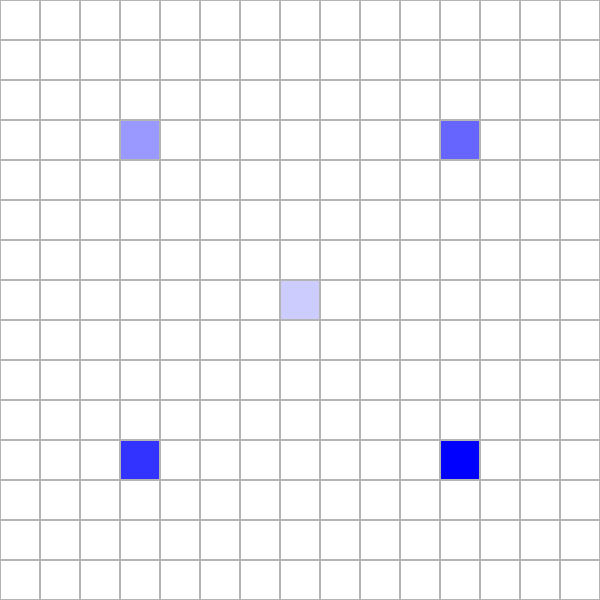
\includegraphics[width=\linewidth*4/5]{grid.png}
		\caption{A simple grid environment that discourages exploration.}
		\label{fig:grid}
	\end{figure}
	
	\section{Model Description}
	
	\section{Data and Experimental Results}
	curiosity found rewards along walls
	
	
	
	
	
	\section{Conclusion and Future Work}
	The conclusion goes here. \cite{lstm}
	
	
	\bibliography{report}{}
	\bibliographystyle{ieeetr}
	
	
	
	%\appendices
	%\section{}
	%Appendix text goes here.
	
	
	% use section* for acknowledgement
	%\ifCLASSOPTIONcompsoc
	% The Computer Society usually uses the plural form
	%  \section*{Acknowledgments}
	%\else
	% regular IEEE prefers the singular form
	%  \section*{Acknowledgment}
	%\fi
	
	
	
	% Can use something like this to put references on a page
	% by themselves when using endfloat and the captionsoff option.
	\ifCLASSOPTIONcaptionsoff
	\newpage
	\fi
	
	
	
\end{document}